%%%%%%%%%%%%%%%%%%%%%%%%%%%%%%%%%%%%%%%%%%%%%%%%%%%%%%%%%%%%%%%%%%%%%%%%%%%

\documentclass{standalone}

\usepackage{amsmath}
\usepackage{mathptmx}
\usepackage{pgfplots}
\usetikzlibrary{external}
\tikzexternalize{vapour-pressure-errors}
\pgfplotsset{compat=1.16}

%% IEEE uses Times Roman font, so we'll default to Times.
%% These three commands make up the entire times.sty package.
\renewcommand{\rmdefault}{ptm}
\renewcommand{\ttdefault}{pcr}
\normalfont\selectfont

\begin{document}

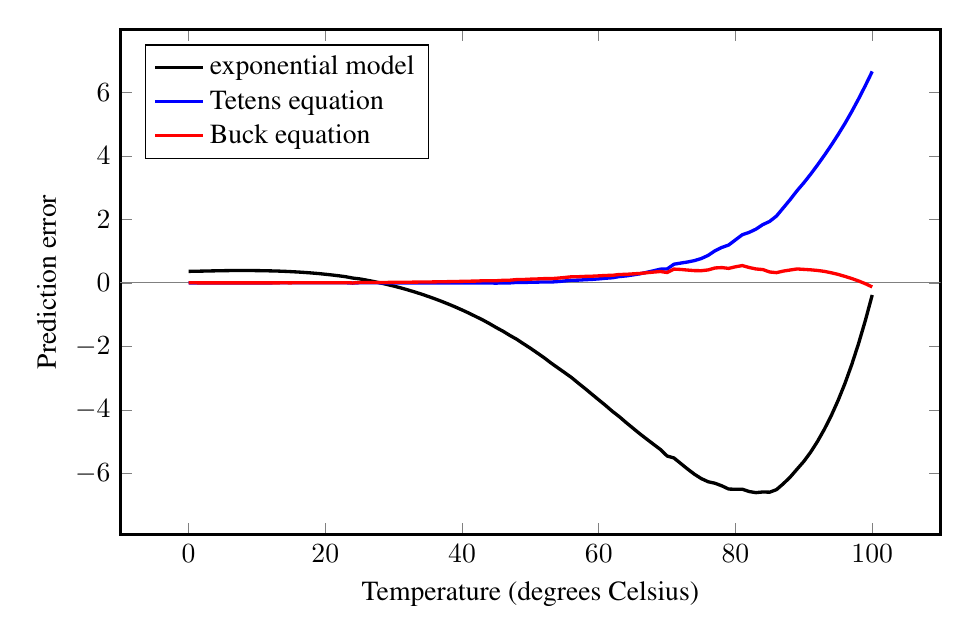
\begin{tikzpicture}
\tikzset{%%
  every mark/.append style={scale=1.0},%%
  scale=1.0%%
}
\pgfplotsset{%%
  every axis/.append style={font=\normalsize}%%
}
%%
\begin{axis}[%%
  axis line style=very thick,%%
  dotStyle/.style={very thick,mark=none},%%
  enlargelimits=true,%%
  height=8cm,%%
  legend cell align=left,%%
  legend pos=north west,%%
  width=12cm,%%
  %% x axis
  xlabel={\normalsize Temperature~(degrees~Celsius)},%%
  %% y axis
  ylabel={\normalsize Prediction error},%%
  scaled y ticks=false,%%
  y tick label style=/pgf/number format/fixed%%
]
%%
%%
%% Horizontal line through origin.
\draw[gray,thin] ({rel axis cs:0,0}|-{axis cs:0,0}) -- ({rel axis cs:1,0}|-{axis cs:1,0});
%%
%%
%% Errors from using a simple exponential model.
\addplot[dotStyle,black] coordinates {
  (0, 0.363090375617866)
  (1, 0.366660196506106)
  (2, 0.371275031129725)
  (3, 0.376135491368398)
  (4, 0.38049679337567)
  (5, 0.384670699649285)
  (6, 0.388027507352721)
  (7, 0.38999808320809)
  (8, 0.390075945259087)
  (9, 0.389819391782922)
  (10, 0.386853677607967)
  (11, 0.383873238073067)
  (12, 0.378643960842137)
  (13, 0.373005505765397)
  (14, 0.364873672956703)
  (15, 0.354242819232182)
  (16, 0.343188323034301)
  (17, 0.328869097940357)
  (18, 0.312530154831643)
  (19, 0.294505212775732)
  (20, 0.272219358650805)
  (21, 0.249191755515497)
  (22, 0.223038399704794)
  (23, 0.194474926608137)
  (24, 0.152319465060302)
  (25, 0.127495540251985)
  (26, 0.089035025042708)
  (27, 0.047081139532988)
  (28, 0.001891498728394)
  (29, -0.047158791894962)
  (30, -0.099573993142229)
  (31, -0.154734541407308)
  (32, -0.215893810803742)
  (33, -0.280174828408157)
  (34, -0.348566942930148)
  (35, -0.421922447148106)
  (36, -0.498953154472957)
  (37, -0.580226930026853)
  (38, -0.666164176646696)
  (39, -0.756034276246979)
  (40, -0.851951986998735)
  (41, -0.950873796805944)
  (42, -1.05759423358044)
  (43, -1.16274213284478)
  (44, -1.28077686320876)
  (45, -1.40598451028971)
  (46, -1.52247401967213)
  (47, -1.65417329951579)
  (48, -1.77482528345114)
  (49, -1.91798395441532)
  (50, -2.0570103301046)
  (51, -2.2050684107421)
  (52, -2.35512108987267)
  (53, -2.51992602892429)
  (54, -2.67203149628696)
  (55, -2.82377217168177)
  (56, -2.97726491661372)
  (57, -3.15440451171325)
  (58, -3.32685936179297)
  (59, -3.50606716946322)
  (60, -3.68323057816346)
  (61, -3.85931278548352)
  (62, -4.04503312766713)
  (63, -4.21086263619767)
  (64, -4.39701956739177)
  (65, -4.57346490592684)
  (66, -4.74989784325342)
  (67, -4.91575123185027)
  (68, -5.08018701629396)
  (69, -5.24209164212701)
  (70, -5.45007144351817)
  (71, -5.51244801072443)
  (72, -5.68725353836524)
  (73, -5.86222615554232)
  (74, -6.02480523883406)
  (75, -6.1621267092126)
  (76, -6.26101831393703)
  (77, -6.30799489448015)
  (78, -6.38925364155648)
  (79, -6.49066933833279)
  (80, -6.4977895928896)
  (81, -6.49583006103438)
  (82, -6.56966966054813)
  (83, -6.60384577795998)
  (84, -6.58254946896432)
  (85, -6.58962065356718)
  (86, -6.50854330708029)
  (87, -6.32244064807162)
  (88, -6.11407032437705)
  (89, -5.86581959830147)
  (90, -5.61970053210519)
  (91, -5.32734517491065)
  (92, -4.99000075212689)
  (93, -4.60852485852922)
  (94, -4.18338065608225)
  (95, -3.70463207764226)
  (96, -3.1719390376436)
  (97, -2.57455265087128)
  (98, -1.91131046043824)
  (99, -1.18063167606431)
  (100, -0.380512423763093)
};
\addlegendentry{exponential model}
%%
%%
%% Errors from using the Tetens equation.
\addplot[dotStyle,blue] coordinates {
  (0, 0.002239677640001)
  (1, -0.000423577706989)
  (2, -0.001412350544507)
  (3, -0.001455177106259)
  (4, -0.00122265802191)
  (5, -0.000325502956196)
  (6, 0.00068746195423)
  (7, 0.001331323608229)
  (8, 0.001187148103952)
  (9, 0.001904083241108)
  (10, 0.001201497014252)
  (11, 0.001871151720128)
  (12, 0.001779413273001)
  (13, 0.002869495292961)
  (14, 0.003163737503703)
  (15, 0.00276591794802)
  (16, 0.003863598501525)
  (17, 0.00373050313773)
  (18, 0.003728928370602)
  (19, 0.004312185274419)
  (20, 0.003027072454657)
  (21, 0.003516379318302)
  (22, 0.003521418967125)
  (23, 0.003884590013161)
  (24, -0.006448033408134)
  (25, 0.00357591582555)
  (26, 0.003117741967042)
  (27, 0.002450356431929)
  (28, 0.001960972906531)
  (29, 0.001153826698424)
  (30, 0.000652917476579)
  (31, 0.001204774529249)
  (32, -0.000318756350559)
  (33, -0.000917705259511)
  (34, -0.001461150782994)
  (35, -0.00268437373861)
  (36, -0.003185993020189)
  (37, -0.003425084512081)
  (38, -0.00371828405715)
  (39, -0.003236875475466)
  (40, -0.004003864641803)
  (41, -0.002891040641792)
  (42, -0.004616025037343)
  (43, 0.000260689719198)
  (44, -0.002661288326948)
  (45, -0.007619270499504)
  (46, 0.0013155003234)
  (47, 0.00024084413478)
  (48, 0.015426643758616)
  (49, 0.013317849262592)
  (50, 0.020537485739496)
  (51, 0.023889663367243)
  (52, 0.030362588657411)
  (53, 0.027131575798677)
  (54, 0.041562057001627)
  (55, 0.061212590749719)
  (56, 0.083837866863647)
  (57, 0.08739170728478)
  (58, 0.100030061488155)
  (59, 0.110113995435995)
  (60, 0.126212672986156)
  (61, 0.14710632867471)
  (62, 0.161789230797183)
  (63, 0.199472633714407)
  (64, 0.219587718320042)
  (65, 0.251788519609875)
  (66, 0.285954840300093)
  (67, 0.332195149452616)
  (68, 0.380849465069616)
  (69, 0.432492219630717)
  (70, 0.437935107557053)
  (71, 0.588229913592329)
  (72, 0.62467132110433)
  (73, 0.658799699323367)
  (74, 0.702403868538966)
  (75, 0.767523842295873)
  (76, 0.866453545636318)
  (77, 1.01174350845275)
  (78, 1.1162035330284)
  (79, 1.1929053348515)
  (80, 1.35518515580901)
  (81, 1.51664634888101)
  (82, 1.59116193346108)
  (83, 1.69287712045923)
  (84, 1.83621180634628)
  (85, 1.93586303531902)
  (86, 2.10680742878418)
  (87, 2.36430358137113)
  (88, 2.62389442270188)
  (89, 2.90140954416592)
  (90, 3.15296748995922)
  (91, 3.42497801166985)
  (92, 3.71414428570677)
  (93, 4.01746509288523)
  (94, 4.33223695950676)
  (95, 4.66605625927798)
  (96, 5.01682127544234)
  (97, 5.39273422251074)
  (98, 5.79230322699732)
  (99, 6.21434426658686)
  (100, 6.65798306716818)
};
\addlegendentry{Tetens equation}
%%
%%
%% Errors from using the Buck equation.
\addplot[dotStyle,red] coordinates {
  (0, 0.005464951980001)
  (1, 0.002392991682726)
  (2, 0.000991210632797)
  (3, 0.000535225676843)
  (4, 0.000359012651337)
  (5, 0.000856869021147)
  (6, 0.001485411299726)
  (7, 0.001765606708618)
  (8, 0.001284838490434)
  (9, 0.00169900424588)
  (10, 0.000734646622238)
  (11, 0.001191115637488)
  (12, 0.000942761881756)
  (13, 0.001941159795159)
  (14, 0.002217360179332)
  (15, 0.00188417105849)
  (16, 0.003138465964797)
  (17, 0.00326351868269)
  (18, 0.003631363447017)
  (19, 0.004705179550946)
  (20, 0.004041699281391)
  (21, 0.005293638062248)
  (22, 0.006212145649329)
  (23, 0.007649277185074)
  (24, -0.001439517113418)
  (25, 0.010007115106792)
  (26, 0.011158951475721)
  (27, 0.012296732797672)
  (28, 0.01381471434912)
  (29, 0.015223229193325)
  (30, 0.017151262099141)
  (31, 0.020349032624786)
  (32, 0.021690585901666)
  (33, 0.024176389628885)
  (34, 0.026935935766147)
  (35, 0.029230345390722)
  (36, 0.032454975164129)
  (37, 0.036142023835041)
  (38, 0.039963137186817)
  (39, 0.044732009822845)
  (40, 0.048406982167499)
  (41, 0.054093631046278)
  (42, 0.057047352199298)
  (43, 0.066675933068581)
  (44, 0.068542114193818)
  (45, 0.068366137541318)
  (46, 0.082028280085737)
  (47, 0.085571370960778)
  (48, 0.105203290488703)
  (49, 0.107299449401893)
  (50, 0.118405246563697)
  (51, 0.12523850350189)
  (52, 0.134691874069134)
  (53, 0.133835227546882)
  (54, 0.149918003519431)
  (55, 0.170371536847085)
  (56, 0.1928113510792)
  (57, 0.195039418655796)
  (58, 0.205046386258289)
  (59, 0.211013763683553)
  (60, 0.221316074625747)
  (61, 0.234522967770943)
  (62, 0.239401286621927)
  (63, 0.264917096487409)
  (64, 0.270237667095557)
  (65, 0.284733409302504)
  (66, 0.297979764395137)
  (67, 0.319759044508061)
  (68, 0.340062222694769)
  (69, 0.359090671223811)
  (70, 0.327257846691595)
  (71, 0.435190920572182)
  (72, 0.423732353852927)
  (73, 0.403941414431188)
  (74, 0.387095635982007)
  (75, 0.384692217027862)
  (76, 0.408449358988946)
  (77, 0.470307542001592)
  (78, 0.482430737351933)
  (79, 0.457207555386276)
  (80, 0.507252327798483)
  (81, 0.54540612324007)
  (82, 0.484737695218144)
  (83, 0.438544361295783)
  (84, 0.42035281264782)
  (85, 0.343919853039552)
  (86, 0.323233066377611)
  (87, 0.372511411969413)
  (88, 0.406205746707713)
  (89, 0.438999273418233)
  (90, 0.425807914647635)
  (91, 0.411780611212407)
  (92, 0.392299544869729)
  (93, 0.362980284520063)
  (94, 0.319671855368938)
  (95, 0.268456730540038)
  (96, 0.205650744674131)
  (97, 0.137802929052214)
  (98, 0.061695267888695)
  (99, -0.025657624596534)
  (100, -0.127008906602669)
};
\addlegendentry{Buck equation}
\end{axis}
\end{tikzpicture}

\end{document}
